\documentclass[letterpaper]{article}
\usepackage{geometry}
\geometry{margin=1.2in}
\usepackage[protrusion=true,expansion=true]{microtype}	
\usepackage[boxruled,linesnumbered,vlined,inoutnumbered]{algorithm2e}
\usepackage{amsmath}
\usepackage{amsthm}
\usepackage{amssymb}
\usepackage{mathtools}
\usepackage{mathrsfs}
\usepackage{soul}
\usepackage{natbib}
\usepackage{rotating}
\usepackage{gensymb}
\usepackage{lscape}
\usepackage{array}
\usepackage{makecell}
\renewcommand\theadalign{bc}
\renewcommand\theadfont{\bfseries}
\renewcommand\theadgape{\Gape[4pt]}
\renewcommand\cellgape{\Gape[4pt]}
\usepackage{courier}
\usepackage{lipsum}
\usepackage{graphicx}
\usepackage{subcaption}
\usepackage[space]{grffile}
\usepackage{xcolor}
\definecolor{light-grey}{rgb}{0.9,0.9,0.9}
\definecolor{dark-red}{rgb}{0.4,0.15,0.15}
\definecolor{dark-blue}{rgb}{0,0,0.7}
\usepackage{environ}
\setcounter{tocdepth}{2}
\renewcommand{\contentsname}{Table of Contents}
\usepackage{hyperref}
\hypersetup{
    colorlinks, linkcolor={dark-blue},
    citecolor={dark-blue}, urlcolor={dark-blue}
}

\setlength{\parskip}{1em}
\newcommand{\HIGHLIGHT}[1]{\textcolor{blue}{\textbf{#1}}}
\newcommand{\TODO}[1]{\textcolor{red}{\textbf{#1}}}

\begin{document}
%-----------------
%	Homework 3
%-----------------
\newpage
\begin{center}
    \begin{Large}
    COMPSCI 589 Homework 3 - Spring 2024
    \end{Large}
    \\
    \HIGHLIGHT{Due April 1, 2024, 11:55 pm Eastern Time}
\end{center}
\addcontentsline{toc}{subsection}{\textbf{Homework 3}}



\vspace{0.25in}
\section{Instructions}

\begin{itemize}
    \item This homework assignment consists of a programming portion. While you may discuss problems with your peers, you must answer the questions on your own and implement all solutions independently. In your submission, do explicitly list all students with whom you discussed this assignment. 
    \item We strongly recommend that you use \LaTeX~to prepare your submission. The assignment should be submitted on Gradescope as a PDF with marked answers via the Gradescope interface. The source code should be submitted via the Gradescope programming assignment as a .zip file. Include with your source code instructions for how to run your code. 
    \item We strongly encourage you to use Python 3 for your homework code. You may use other languages. In either case, you \textit{must} provide us with clear instructions on how to run your code and reproduce your experiments. 
    \item You may \textit{not} use any machine learning-specific libraries in your code, e.g., TensorFlow, PyTorch, or any machine learning algorithms implemented in scikit-learn (though you may use other functions provided by this library, such as one that splits a dataset into training and testing sets). You may use libraries like numpy and matplotlib. If you are not certain whether a specific library is allowed, do ask us.
    \item All submissions will be checked for plagiarism using two independent plagiarism-detection tools. Renaming variable or function names, moving code within a file, etc., are all strategies that \textit{do not} fool the plagiarism-detection tools we use. \textcolor{red}{If you get caught, all penalties mentioned in the syllabus \textit{will} be applied---which may include directly failing the course with a letter grade of ``F''}.

    \begin{center}
    \textcolor{red}{$\rightarrow$ Before starting this homework, please review this course's policies on plagiarism by  \\reading Section 14 of the \href{https://people.cs.umass.edu/~bsilva/courses/CMPSCI_589/Spring2024/S24_589_Syllabus_v2.0.pdf\#page=5}{\textcolor{red}{\underline{syllabus}}}.}
    \end{center}

    \item The tex file for this homework (which you can use if you decide to write your solution in \LaTeX), as well as the datasets and starting source code, can be found \href{https://people.cs.umass.edu/~bsilva/courses/CMPSCI_589/Spring2024/homeworks/hw3.zip}{here}.

    \item The automated system will not accept assignments after 11:55 pm on April 1st.    
\end{itemize}
\newpage

\vspace{1cm}
\section*{Programming Section (100 Points Total)}

In this homework, you will be implementing the Random Forest algorithm. \textbf{Notice that you may \ul{not} use existing machine learning code for this problem: you must implement the learning algorithm entirely on your own and from scratch.} 

%--------------------------------------------

In this assignment, you will:

\begin{itemize}
\item Implement the standard Decision Tree algorithm based on the Information Gain splitting criterion. Notice that you must reuse \textbf{\textcolor{red}{\textit{your}}} previous implementation of this algorithm. \HIGHLIGHT{Important: your implementation of the Decision Tree algorithm should support both categorical \textit{and} numerical attributes}. When determining the numerical threshold that should be used when splitting numerical nodes, you may \textit{(i)} use the average of that attribute's values in the partition of instances associated with the current node; or \textit{(ii)} use the more sophisticated (and ``powerful'') technique discussed in lecture 04 (see slide \#66). 
\item Implement a procedure to create bootstrap datasets by sampling (\textit{with replacement}) from the current training set to construct the datasets based on which each tree in the random forest will be trained. 
\item Implement a mechanism to select (whenever a node is being split) $m$ attributes at random from the complete set of attributes of an instance. You should then split the node based on the attribute with the best Information Gain. As a heuristic, we usually use $m \approx \sqrt{X}$, where $X$ is the total number of attributes composing each instance in the dataset.
\item Implement a majority voting mechanism that takes into account the predictions made by each tree in the ensemble to classify new instances.
\item Implement the \textit{stratified cross-validation} technique to evaluate the generalization capability of the random forest. For an example, see Figure~\ref{fig:cross-val}. We recommend using $k=10$ folds. Out of these, $k-1$ folds will be used to train a random forest composed of $ntree$ trees. Here, \textbf{$ntree$ will be the main adjustable hyper-parameter of your algorithm}. The remaining fold---the one not used during training---will be used to evaluate the performance of the random forest itself (\textcolor{red}{i.e., \underline{not} the performance of any individual tree separately!}). This process implies, in particular, that at each step of the cross-validation process, you will be training not only \textit{one} decision tree, but multiple ($ntree$) decision trees, all of which will be combined to compose your random forest. You will then repeat this process, thereby generating (and evaluating) $k$ random forests. The final performance is the average of the performances computed for each of the folds.
\item Evaluate the impact that the number of trees (i.e., the $ntree$ hyper-parameter) has on the performance of your random forest.


\end{itemize}



\section{Deliverables}

The main objective of this homework is to study the impact of the number of trees composing a random forest (i.e., the $ntree$ hyper-parameter) on its performance. When constructing each tree in the ensemble, you are free to choose between many stopping criteria. You may, for instance, \textit{(1)} stop splitting nodes whenever the data partition associated with the current node contains less than $n$ instances---for some $n$ that you pick empirically. We will refer to this as the \texttt{minimal\_size\_for\_split} criterion; \textit{(2)} stop splitting nodes whenever the information gain resulting from a split is not sufficiently high (even though it may be slightly higher than zero). You are free to empirically pick the minimum information gain that you'd like to use. We will refer to this as the 
\texttt{minimal\_gain} criterion; \textit{(3)} stop splitting whenever the current branch of the tree becomes too deep---i.e., its depth becomes larger than some pre-defined value selected empirically by you. We will refer to this as the \texttt{maximal\_depth}  stopping criterion. You are free to choose which criterion (or criteria---you may combine them) you would like to use. \HIGHLIGHT{In all questions below, do not forget to mention explicitly which criterion/criteria you used and what was its corresponding hyper-parameter. We encourage you to try different possibilities to identify the setting that produces the best possible performance for your algorithm.}

\vspace{2cm}

    \begin{figure}[hb!!]
        \centering
        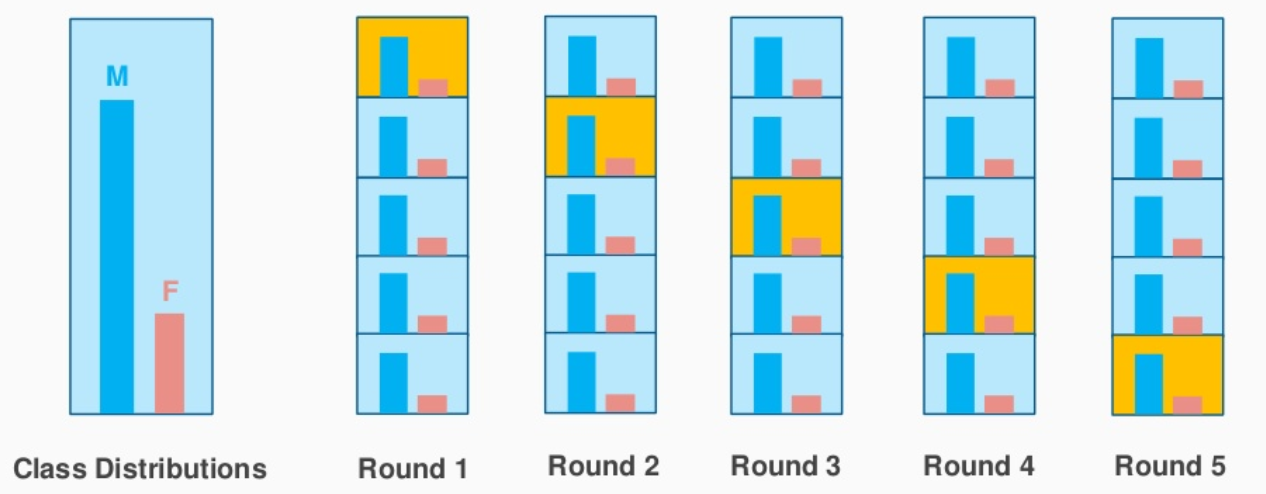
\includegraphics[width=0.85\textwidth]{figures/cross_val_stratified2.png}
        \caption{Example of how to construct \textit{stratified} folds to perform k-fold cross-validation. Here, we assume two classes: ``M'' and ``F''. Notice how the complete dataset (shown in the leftmost figure) is not balanced: approximately 3/4 of its instances belong to the class ``M'', and approximately 1/4 of its instances belong to the class ``F''. We wish to approximately preserve these proportions (i.e., the proportion of instances of class ``M'' and the proportion of instances of class ``F'') in each of the $k=5$ folds. To do this, you should first split the original dataset, $D$, into two: one containing only instances of class ``M'' (sub-dataset $D_M$), and another one containing only instances of class  ``F'' (sub-dataset $D_F)$. Then, given the total number of instances in the original dataset ($D$) and the number of folds you are using ($k$), you should be able to determine the size of each fold. Let us assume that each fold, in this example, should have $50$ instances. To construct it, you should draw random instances from $D_M$ and $D_F$. In this example, 3/4 of the instances that you add to the current fold should come from $D_M$, and 1/4 of the instances that you add to the current fold should come from $D_F$. Notice that because the folds should be disjoint (i.e., an instance should appear in only one fold), after drawing an instance either from $D_M$ or $D_F$, it should be removed from such a set to ensure that it will not be accidentally included as part of another fold. \textit{(Source: \href{https://stats.stackexchange.com/questions/49540/understanding-stratified-cross-validation}{Stack Exchange})}.}
        \label{fig:cross-val}
    \end{figure}

\clearpage
In this homework you will be analyzing two \href{https://people.cs.umass.edu/~bsilva/courses/CMPSCI_589/Spring2024/homeworks/hw3.zip}{datasets}:

\textbf{(1) The Wine Dataset.}
The goal, here, is to predict the type of a wine based on its chemical contents. The dataset is composed of 178 instances. Each instance is described by 13 \textit{numerical} attributes, and there are 3 classes.

\textbf{(2) The 1984 United States Congressional Voting Dataset.}
The goal, here, is to predict the party (Democrat or Republican) of each U.S. House of Representatives Congressperson. The dataset is composed of 435 instances. Each instance is described by 16 \textit{categorical} attributes, and there are 2 classes.


For each dataset, you should:

\begin{enumerate}
    \item Train a random forest and evaluate it using the stratified cross-validation technique discussed above. You should train random forests using different values for the $ntree$ parameter: 1, 5, 10, 20, 30, 40, and 50.
    \item For each value of $ntree$, you should measure the accuracy, precision, recall, and F1 score of the resulting random forest. 
    \item You should then create, for each dataset and for each of the metrics described above, a graph where you show the value of $ntree$ on the x-axis, and where you show the value of the corresponding metric on the y-axis. For example, you should have one graph showing the accuracy of the random forest as a function of $ntree$ for the dataset \#1; another graph showing the precision of the random forest as a function of $ntree$ for the dataset \#1; and similar types of graphs for the other metrics and for dataset \#2. \HIGHLIGHT{These analyses should result in a total of 8 graphs. Please indicate clearly, in the caption of each figure/graph, which results you are presenting in the corresponding figure}.
    \item For each metric being evaluated (and for each dataset), discuss which value of $ntree$ you would select if you were to deploy this classifier in real life. Explain your reasoning. 
    \item Discuss (on a high level) which metrics were more directly affected by changing the value of $ntree$ and, more generally, how such changes affected the performance of your algorithm. For instance: was the accuracy of the random forest particularly sensitive to increasing $ntree$ past a given value? Was the F1 score a  ``harder'' metric to optimize, possibly requiring a significant number of trees in the ensemble? Is there a point beyond which adding more trees does not improve performance---or makes the performance worse?
\end{enumerate}

\vspace{1cm}
\noindent\rule{\textwidth}{1pt}

\textbf{There are three ways in which we may receive extra credit in this homework.}

\noindent \HIGHLIGHT{(Extra Points \#1: 8 Points)} Reconstruct the same graphs as above, but now using the Gini criterion. You should present the same analyses and graphs mentioned above. Discuss whether (and how) different performance metrics were affected (positively or negatively) by changing the splitting criterion, and explain why you think that was the case.

\noindent \HIGHLIGHT{(Extra Points \#2: 8 Points)}
Analyze a third dataset: the \textbf{Breast Cancer Dataset}. The goal, here, is to classify whether tissue removed via a biopsy indicates whether a person may or may not have breast cancer. There are 699 instances in this dataset. Each instance is described by 9 \textit{numerical} attributes, and there are 2 classes. You should present the same analyses and graphs as discussed above. This dataset can be found in the same zip file as the two main datasets.


\noindent \HIGHLIGHT{(Extra Points \#3: 12 Points)}    
Analyze a fourth, more challenging dataset: the \textbf{Contraceptive Method Choice Dataset}. The goal, here, is to predict the type of contraceptive method used by a person based on many attributes describing that person. This dataset is more challenging because it combines \textit{both numerical and categorical attributes}. There are 1473 instances in this dataset. Each instance is described by 9 attributes, and there are 3 classes. The dataset can be downloaded \href{https://archive.ics.uci.edu/ml/datasets/Contraceptive+Method+Choice}{here}. You should present the same analyses and graphs discussed above.

\end{document}






